\title{State Machines in VHDL}
\begin{document}
\section{State Minimization}

\begin{frame}{State minimization}
  State machine are complex enough.  Clearly we don't want to have duplicate states.
  \begin{block}{Conditions for State Minimization}
    Given states S1 and S2:
    \begin{itemize}
      \item S1 and S2 produce the same state machine output values.
      \item For each input combination, S1 and S2 produce the same or equivalent next states.
    \end{itemize}
  \end{block}
  If both conditions are true, then S1 and S2 can be represented by one state.
\end{frame}

\begin{itemize}
  \item This is often necessary after initial design, because initial design is somewhat like brainstorming.
  \item There are formal procedures and tools to do this, but they are beyond the scope of this course.
  \item Sometimes state minimization is not desirable.
\end{itemize}

\section{Decomposing State Machines}

\begin{frame}{Decomposing state machines}
  Often it is useful to think of a complex state machine as multiple simpler state machines that interact.
  \begin{block}{Benefits of state machine decomposition}
    \begin{itemize}
      \item We tend to understand simpler concepts in exponentially shorter time.
      \item Decomposition allows mutliple designers to work in parallel on parts of a state machine independently.
      \item Each component can be tested independently.
    \end{itemize}
  \end{block}
  A common way to decompose a state machine is to separate it into a main machine and a counter.
\end{frame}

\begin{frame}{Decomposed design example}
  \begin{center}
    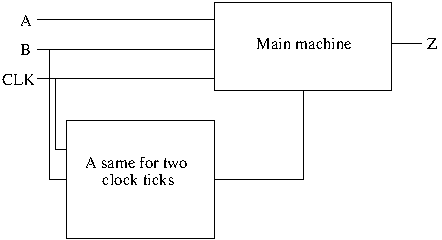
\includegraphics[scale=1.3]{DecomposedStateMachine}
  \end{center}
\end{frame}

\section{State Machines in VHDL}

\begin{frame}{The event attribute}
  \begin{definition}
    In VHDL, the \alert{event} attribute of a signal is a boolean which is true when the value of the signal changes to trigger a process statement.
  \end{definition}
  \begin{block}{Using a clock signal in a process statement}
    We can check for a rising or falling clock signal list this:
    \begin{itemize}
      \item \texttt{if CLK'event and CLK='1' then RISING\_EDGE='1';}
      \item \texttt{if CLK'event and CLK='0' then FALLING\_EDGE='1';}
    \end{itemize}
  \end{block}
  You will often see this in clocked synchronous state machine designs.
\end{frame}

\begin{frame}{VHDL state machine structure}
  A state machine in VHDL is usually divided into three \texttt{process} statements.
  \begin{itemize}
    \item State memory (clock signal)
    \item Next-state excitation logic (current state and inputs)
    \item Output logic (current state and inputs)
  \end{itemize}
\end{frame}

\subsection{State Table Design}

\begin{frame}{VHDL state table design}
  If a state table it available, then it can be directly translated to VHDL, as in the following example.
\end{frame}

Show VHDL from table 7-38.

\subsection{Direct State Machine Design}

\begin{frame}{VHDL direct state machine design}
  If a state table has not been determined, it is often possible to move directly from the problem statement to the VHDL code, as in the following example.
\end{frame}

\end{document}
